\documentclass[a4paper]{article}

%% Language and font encodings
\usepackage[spanish]{babel}
\usepackage[utf8x]{inputenc}
\usepackage[T1]{fontenc}
\usepackage{listings}
\spanishdecimal{.}


%% Sets page size and margins
\usepackage[a4paper,top=3cm,bottom=2cm,left=3cm,right=3cm,marginparwidth=1.75cm]{geometry}

%% Useful packages
\usepackage{amsmath}
\usepackage{graphicx}
\usepackage[colorinlistoftodos]{todonotes}
\usepackage[colorlinks=true, allcolors=blue]{hyperref}

\title{Práctica 1: movimiento Browniano}
\date{}
\begin{document}

\maketitle

\section{Introducci\'on}
En esta práctica se observa el movimiento que realiza una partícula a travez de diferentes planos de movimiento, dicho movimiento lo realiza con una aleatoriedad, lo cual se conoce como movimiento Browniano, la intención será en primer momento conocer la probabilidad con la cual la partícula regresará a su punto de salida, tomando éste como el origen, así mismo los retos adicionales nos ayudarán a contabilizar los tiempos que tarda el programa en realizar una caminata, así como los tiempos que tardaría si no tuviéramos una versión paralela, intentando visualizar la ventaja o desventaja que la paralelización representa en esta práctica.
\section{Par\'ametros de trabajo}
La experimentación se realizó en un HP Z230 Tower Workstation con procesador Intel(R) Xenon(R) CPU E3-1240 v3 y 3.40 GHz de memoria ram 16 GB y un sistema operativo de 64 bits con Windows 7 Home Premium.

Se simulan caminatas de una partícula a través de $8$ dimensiones, con un largo de pasos en las caminatas de $p \in \{50,80,150,200,400\}$ y una repetición de $\{100, 300\}$. La cantidad de dimensión para la tarea original se mantienen como se mencionó anteriormente para la práctica original, ya que para los retos se aumenta hasta $10$ dimensiones con el fin de observar si existe algun cambio significativo en los tiempos de ejecución, así como se aumentaron la cantidad de pasos, ya que los mismos parámetros para la práctica original no causaban efecto significativo en los tiempos de ejecución, los pasos que se usaron para los retos fueron $p \in \{500,800,2000,10000\}$, las cantidad de repeticiones se mantuvieron en $100$ para ambos retos.

\section{Modificaciones del código}
Se agregaron para la práctica un ciclo \texttt{for} que nos ayudara a variar de forma automática la cantidad de pasos que realiza en cada caminata, así mismo fue agregado un \texttt{vector} el cual guarda las cantidades a variar. Para generar las imágenes fue necesario incluir la librería \texttt{ggplot}.

\begin{lstlisting}[frame=single]
library('ggplot2')
...
d <- c(500,800,2000,10000)
...
for (l in 1:length(d)){
duracion <- d[l]
}
\end{lstlisting}

Para la generación de las imágenes que comparan tanto los tiempos como la cantidad de veces que la partícula llega al origen se utilizó una linea similar.
\begin{lstlisting}[frame=single]
png(paste("DimEuN.png", sep=""), width=700, height=700)
ggplot(data=datos,aes(x=Dimension,y=Tiempo,fill=Pasos))+geom_boxplot()
+xlab("Dimensi\u{F3}n")+ ylab("Tiempo de ejecuci\u{F3}n (s)")
graphics.off()
\end{lstlisting}

\section{Resultados y conclusiones}
En la figura \ref{fig:PorcentajesEu} se puede observar que la cantidad de veces que una partícula llega al origen sin importar la cantidad de pasos es sumamente superior cuando solo se tiene una dimensión. Al ir incrementando la cantidad de dimensiones este porcentaje va disminuyendo drásticamente.

\begin{figure}[h]
\centering
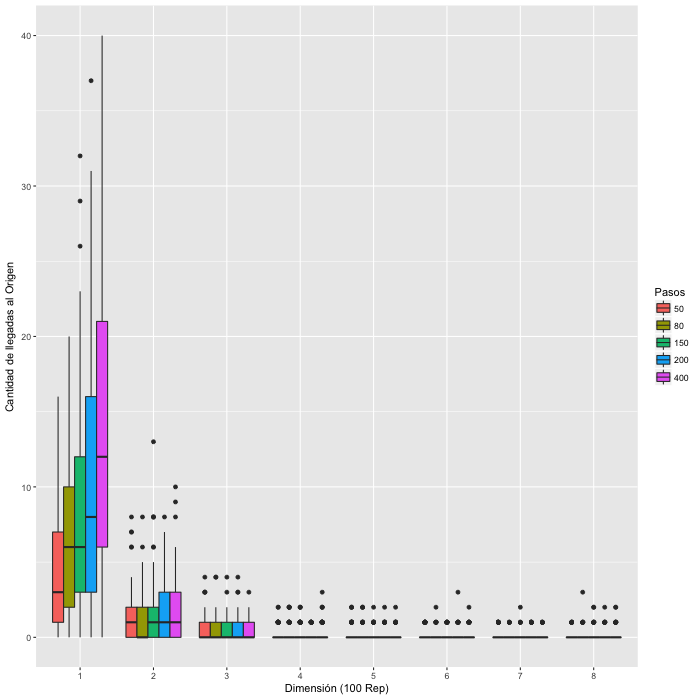
\includegraphics[width=0.7\linewidth]{PorcentajesEu}
\caption{Porcentaje de llegada al origen referente a la cantidad de dimenciones de movimiento de la partícula.}
\label{fig:PorcentajesEu}
\end{figure}

De igual forma al aumentar la cantidad de repeticiones en la experimentación los gráficos muestran un comportamiento prácticamente idéntico, es decir es muy evidente en la figura \ref{fig:PorcentajesEu300} observar que el número de repeticiones no tienen un efecto significativo en la experimentación, así como es evidente que el factor que más aumenta la probabilidad de regresar al origen al estar en una sola dimensión.
\begin{figure}
\centering
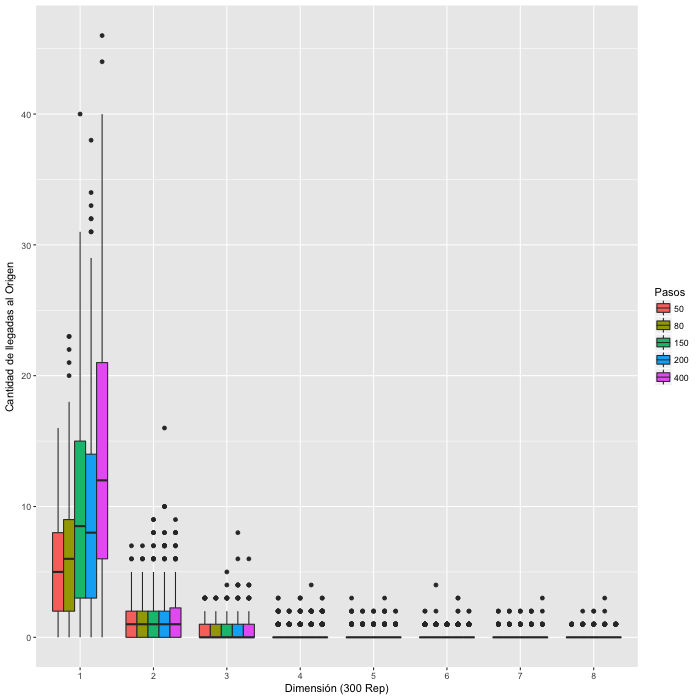
\includegraphics[width=0.7\linewidth]{PorcentajesEu300}
\caption{Cantidad de veces que la partícula llegó al origen con 300 repeticiones.}
\label{fig:PorcentajesEu300}
\end{figure}

\section{Reto 1}
El reto uno consiste en medir los tiempos de ejecución de las caminatas variando la cantidad de pasos, así como la dimensión en el movimiento de la partícula

\section{Modificación del código y parámetros de R1}
Fue necesario agregar las funciones que te ayudan a medir el tiempo de ejecución así como agregar el comando que te permite observar dichos tiempos en segundos. Se agregaron los gráficos de los tiempos, así comopara que variaran por largo de caminata y por dimensión.
\begin{lstlisting}[frame=single]
     c <- Sys.time()
      d <- Sys.time()
      ti <- c(c,d)
      tie <- diff(ti,units="secs")
      todo <- c(duracion,dimension,mayor,tie)
      ....
###Largo de la caminata##
png(paste("LargoEu.png", sep=""), width=700, height=700)
ggplot(data=graficas,aes(x=Pasos,y=Tiempo,fill=Dimension))+
geom_boxplot()+xlab("Largo de la Caminata")+
ylab("Tiempo de ejecuci\u{F3}n (s)")
graphics.off()
\end{lstlisting}
\section{Resultados y conclusiones de R1}

\section{Reto 2}


\section{Modificación de código y parámetros R2}

\section{Resultados y conclusiones de R2}

\end{document}